%---------- Inleiding ---------------------------------------------------------

\section{Introductie}%
\label{sec:introductie}

Bedrijven merken het laatste jaar op dat hun maandelijkse energiefactuur begint te stijgen, een van de reden hiervoor is dat bedrijven veel vaker elektrische wagens aankopen, omdat deze aankoop fiscaal voordeliger is. Elektrische wagens zijn, momenteel, namenlijk 100\% fiscaal aftrekbaar volgens \textcite{Blomme2023}. De tweede reden is een gevolg van het aankopen van elektrische wagens, zo kunnen bedrijven ook laadpalen voor deze wagens aankopen. Dit gebeurt zodat de werknemers hun wagens op de plaats waar het bedrijf gevestigd is, kunnen laden. Vooral de tweede reden heeft invloed op de bedrijven, omdat hoe meer laadpalen er gebruikt worden, hoe meer elektriciteit er verbruikt wordt. Bovenop de vorige twee redenen, dienen bedrijven vanaf werkjaar 2023 een toegangsvermogen te bepalen. Dit toegangsvermogen uitgedrukt in kilowatt, is een eigen inschatting van je maandelijkse piekvermogen \autocite{Fluvius2022}. Het maandelijkse piekvermogen bevat het kwartier in de maand met het hoogste verbruik, anders verwoord is dit het hoogste gemiddelde vermogen, gemeten in een kwartier \autocite{Fluvius2022}. Volgens \textcite{Fluvius2022} wordt er een boete aangerekend waneer het werkelijk maandelijkse piekvermogen hoger ligt dan de eigen opgegeven toegangsvermogen. Dit bedrag is gebaseerd op het verschil tussen de te hoge piekvermogen en het doorgegeven toegangsvermogen. Die waarde in kilowatt wordt dan 12 maanden lang aangerekend volgens een tarief dat 50\% hoger ligt dan het toegangsvermogen.

Dit geldt ook voor Carwash Clean Car, een kleine zelfstandige, gelegen te Dendermonde. De eigenaar van deze carwash zoekt hierdoor een oplossing om zijn maandelijkse energiefactuur te verlagen. De eigenaar heeft al een aantal maatregelen genomen om de energiefactuur te verlagen, zo zijn er al zonnepanelen geplaatst, de auto's worden enkel ingestoken als de zon schijnt of na 22 uur 's avonds, omdat er dan gebruik wordt gemaakt van het nachttarief... Maar de wagens enkel laden als de zon schijnt helpt niet echt om de energiefactuur te verlagen, omdat soms vergeten wordt de lader los te koppelen van de wagen. Daarom wordt er in deze bachelorproef onderzoek gedaan om de vraag te beantwoorden: "Hoe kan het maandelijks elektrisiteitsverbruik van het bedrijf Carwash Clean Car gemonitord worden om zo het verbruik van de laadpalen voor auto's te optimaliseren door middel van het slim aansturen van deze laadpalen met behulp van een custom geschreven applicatie?".

Als het onderzoek succesvol is, kan de eigenaar van Carwash Clean Car zijn laadpalen voor auto's laten aansturen via een custom geschreven applicatie om zo het energieverbruik te optimaliseren. Dit onderzoek zal hier een antwoord op bieden aan de hand van een literatuurstudie, waar er verschillende technologieën worden bekeken, welke connecties moeten gemaakt worden om de juiste dataregisters aan te spreken van de laadpalen en monitoring van het energieverbruik. Na de literatuurstudie wordt er een proefopstelling opgesteld om de gevonden informatie toe te passen, om zo een progressive web app te maken voor het bedrijf.

%---------- Stand van zaken ---------------------------------------------------

\section{literatuurstudie}%
\label{sec:literatuurstudie}

\subsection{Inleiding}%
\label{sub:inleiding_literatuurstudie}
In dit deel van het voorstel van het vooorstel zijn er bronnen gezocht om een voorkennis te hebben over laadpalen voor wagens en het monitoren van de opgewekte energie van de zonnepanelen. Er wordt ook gekeken naar de benodigdheden om de laadpalen aan te sturen en de dataregisters uit te lezen. Als laatste wordt er gekeken naar de mogelijkheden om een progressive web app te maken.

\subsection{Modbus protocol}%
\label{sub:modbus_protocol}
Het Modbus protocol is een communicatieprotocol dat gebruikt wordt om dataregisters uit te lezen van verschillende apparaten. Het protocol was origineel geïmplementeerd als een applicatie-level protocol dat gebruikt zou worden om data te versturen over een seriële laag, maar is ondertussen uitgebreid naar implementaties over seriële, TCP/IP en de user datagram protocol (UDP) \autocite{NI2023}. Met dit protocol kunnen er verschillende dataregisters uitgelezen worden, zoals de status van de laadpaal, het verbruik van de laadpaal, de spanning van de laadpaal, de energie dat zonnepanelen momenteel opbrengen. Het protocol zal gebruikt worden om de dataregisters uit te lezen en opdrachten te versturen naar de laadpalen.

\subsection{Backend}%
\label{sub:backend}
De backend van de applicatie zal geschreven worden in Node-RED. Node-RED is een visuele tool die gebruikt wordt om applicaties te maken door middel van het verbinden van verschillende nodes. Deze nodes kunnen verschillende taken uitvoeren, zoals het versturen van een e-mail, het versturen van een HTTP request, ... Hier wordt Node-RED gebruikt om de dataregisters uit te lezen van de laadpalen en zonnepanelen. Deze data wordt dan opgevraagd door de progressive web app. De progressive web app zal dan op zijn beurt de data gebruiken om de laadpalen aan te sturen.

\subsection{Progressive web app}%
\label{sub:progressive_web_app}
De progressive web app zal geschreven worden in ReactJS. ReactJS is een JavaScript library die gebruikt wordt om user interfaces te maken. De progressive web app zal gebruik maken van de data die opgevraagd wordt door de backend om de laadpalen aan te sturen. Deze data van de zonnepanelen zal in een grafiek gegoten worden zodat de eigenaar een idee heeft van hoeveel energie er wordt verbruikt en hoeveel energie er wordt opgewekt. De progressive web app zal ook een overzicht geven van de laadpalen, waar de eigenaar de laadpalen kan aansturen.

\subsection{Dataregisters}%
\label{sub:dataregisters}
Online zijn er lijsten te vinden over de dataregisters van de laadpalen en zonnepanelen. Voor deze bachelorproef wordt er gebruik gemaakt van lijst die beschikbaar is op de website van \textcite{Alfen2020}. De lijst van de dataregisters van de zonnepanelen staat op de website van \textcite{solarinverters2016}.

% Voor literatuurverwijzingen zijn er twee belangrijke commando's:
% \autocite{KEY} => (Auteur, jaartal) Gebruik dit als de naam van de auteur
%   geen onderdeel is van de zin.
% \textcite{KEY} => Auteur (jaartal)  Gebruik dit als de auteursnaam wel een
%   functie heeft in de zin (bv. ``Uit onderzoek door Doll & Hill (1954) bleek
%   ...'')

%---------- Methodologie ------------------------------------------------------
\section{Methodologie}%
\label{sec:methodologie}

\subsection{literatuurstudie}%
\label{sub:literatuurstudie_methodologie}
Om het onderzoek te starten wordt er eerst een literatuurstudie gedaan. Hierbij wordt er meer informatie gezocht over de verschillende apparaten die nodig zijn om het onderzoek succesvol te laten verlopen. Er wordt ook gekeken naar de verschillende technologieën die gebruikt kunnen worden om de laadpalen aan te sturen en de dataregisters uit te lezen. Deze informatie komt uit wetenschappelijke artikels en de documentatie van de technologieën. De voorkennis dat er verkregen is, is dan ook de einddeliverable van deze literatuurstudie. Het opstellen van de literatuurstudie gebeurt in de eerste 3 weken van het onderzoek.

\subsection{Selectie van de technologieën}%
\label{sub:selectie_van_de_technologieen}
Aan de hand van de literatuurstudie wordt er een selectie gemaakt van de technologieën die gebruikt zullen worden in het onderzoek. Er wordt gekeken naar welke technologieën het meest geschikt zijn voor het onderzoek en de haalbaarheid van de implementatie. De einddeliverable van deze fase is een lijst met de technologieën die gebruikt zullen worden in het onderzoek. Deze fase wordt uitgevoerd in de 4de week van het onderzoek.

\subsection{Opstellen van de proefopstelling}%
\label{sub:opstellen_van_de_proefopstelling}
Na de selectie van de technologieën wordt er een proefopstelling opgesteld. Hierbij wordt er progressive web app gemaakt die de laadpalen kan aansturen in het lokale netwerk. De progressive web app zal ook de data van de zonnepanelen uitlezen, om zo de laadpalen te kunnen aansturen. Naast de progressive web app zal er ook een backend applicatie geschreven worden die de verzoeken afhandelt tussen de progressive web app en de laadpalen. De einddeliverable van deze fase is een werkende proefopstelling. Deze fase wordt uitgevoerd in de 5de tot en met de 9de week van het onderzoek.

\subsection{conclusie}%
\label{sub:conclusie_methodologie}
Na het opstellen van de proefopstelling wordt er een conclusie geschreven. Hierbij wordt er gekeken of de proefopstelling voldoet aan de verwachtingen en de doelstellingen van het onderzoek. De einddeliverable van deze fase is een conclusie. Deze fase wordt uitgevoerd in de 10de week van het onderzoek.


\begin{figure}[b]
  \centering
  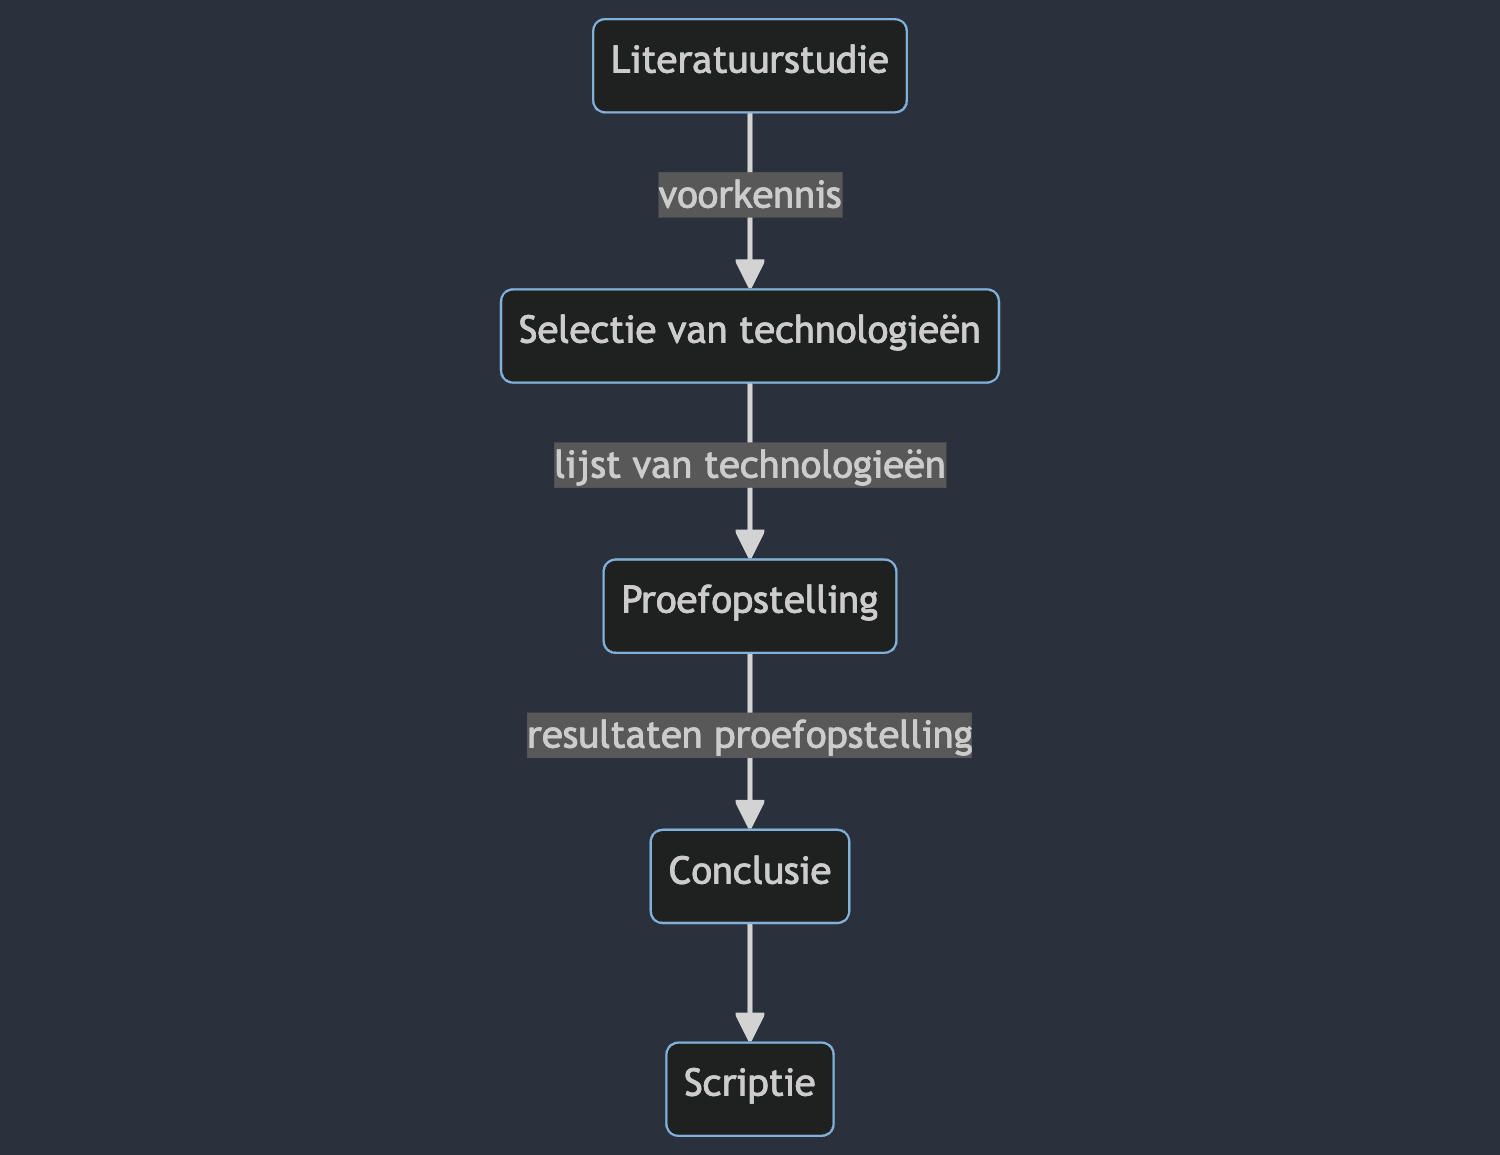
\includegraphics[width=0.35\textwidth,height=0.35\textheight,keepaspectratio]{./graphics/mermaid-diagram.png}
  \caption{flowchart diagram van de methodologie.}
  \label{fig:flowchart}
\end{figure}

\newpage
%---------- Verwachte resultaten ----------------------------------------------
\section{Verwacht resultaat, conclusie}%
\label{sec:verwachte_resultaten}

\subsection{Verwacht resultaat}%
\label{sub:verwacht_resultaat}
De verwachte resultaten van het onderzoek zijn dat het elektriciteitsverbruik van het bedrijf Carwash Clean Car meer afgevlakt wordt, dit kan door het monitoren en beheren van hun elektriciteitsverbruik. Hierbij kan er gezien worden hoeveel energie er wordt aangekocht. Deze gegevens kunnen geanalyseerd worden, om zo de elektrische voertuigen automatisch van het bedrijf te laten laden wanneer er groene energie over is.

\subsection{Conclusie}%
\label{sub:conclusie}
De conclusie van het onderzoek is dat het mogelijk is om het elektriciteitsverbruik van het bedrijf Carwash Clean Car te monitoren en te beheren. Dit kan door het monitoren van de dataregisters van de laadpalen en de zonnepanelen. De dataregisters van de laadpalen en de zonnepanelen kunnen uitgelezen worden door middel van het Modbus protocol. De dataregisters van de laadpalen en de zonnepanelen kunnen uitgelezen worden door middel van een backend applicatie die geschreven is in Node-RED. De progressive web app zal de data van de laadpalen en de zonnepanelen gebruiken om de laadpalen aan te sturen. De progressive web app zal geschreven worden in ReactJS.